\documentclass{cv}

% Graphics and images
\usepackage{graphicx}
% Encodings (to render letters with diacritics and special characters)
\usepackage[utf8]{inputenc}
\usepackage[T1]{fontenc}
% Language
\usepackage[portuguese]{babel}

% Document
\begin{document}
\thispagestyle{empty}
\noindent
\begin{minipage}[l]{0.75\textwidth}
	\section*{Diogo Miguel Ferreira Rodrigues}
	%Rua de Avioso, 553 | Castêlo da Maia (4475-617 MAIA)\\
    Maia, Portugal\\
    \begin{tabular}{@{}c @{\hskip 0.5em} l @{\hskip 5em} c @{\hskip 0.5em} l @{}}
        
\includegraphics[height=7px]{img/email.png}    & \href{mailto:diogo.rodrigues@fe.up.pt}{diogo.rodrigues@fe.up.pt}     & 
\includegraphics[height=7px]{img/linkedin.png} & \href{https://www.linkedin.com/in/dmfrodrigues/}{dmfrodrigues} \\
                                                       & \href{mailto:dmfrodrigues2000@gmail.com}{dmfrodrigues2000@gmail.com} & 
\includegraphics[height=7px]{img/github.png}   & \href{https://github.com/dmfrodrigues}{dmfrodrigues}\\
        %
\includegraphics[height=7px]{img/phone.png}    & +351 915507239 \\
    \end{tabular}
\end{minipage}%
\begin{minipage}[l]{0.24\textwidth}
	\begin{center} 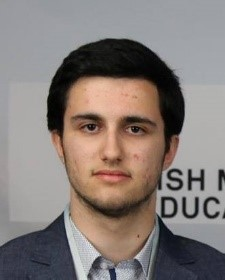
\includegraphics[height=30mm]{img/cv_photo.jpg} \end{center}
\end{minipage}
\subsection*{Education}
\job{Master in Informatics and Computing Engineering}{2021 – 2023}{
Faculty of Engineering of the University of Porto
}
\job{Bachelor in Informatics and Computing Engineering}{2018 – 2021}{
Faculty of Engineering of the University of Porto\\
Final grade: 18.92/20.00
}
\job{Secondary School – Sciences and Technologies Programme (10th-12th grade)}{2015 – 2018}{
Castêlo da Maia Secondary School (ESCM)\\
Final grade: 19.6/20.0\\
Matematics National Exam (12th grade): 18.8/20.0\\
Physics and Chemistry National Exam (11th grade): 19.5/20.0\\
Portuguese Language National Exam (12th grade): 16.5/20.0\\
Biology and Geology National Exam (11th grade): 17.5/20.0\\
Optional subjects (12th grade): Physics, Informatics\\
Specific subjects (10th/11th grades): Physics and Chemistry, Biology and Geology\\
Excelence Board on school years 2015/16, 2016/17 and 2017/18\\
Merit Board on school year 2017/18\\
Merit Prize from the Ministry of Education, for best grade of the school
}
\job{3rd cycle of Basic Education (7th-9th grade)}{2012 – 2015}{
Castêlo da Maia Basic School of 2nd and 3rd Cycles (EB2/3 Castêlo da Maia) – 7th grade\\
Castêlo da Maia Secondary School (ESCM) – 8th/9th grades\\
Final grade: 5.0/5.0\\
First foreign language: English\\
Second foreign language: French\\
Excelence Board on school years 2012/13, 2013/14 and 2014/15
}
\job{2nd cycle of Basic Education (5th-6th grade)}{2010 – 2012}{
Castêlo da Maia Basic School of 2nd and 3rd Cycles (EB2/3 Castêlo da Maia)\\
Final grade: 5.0/5.0\\
Excelence Board on school years 2010/11 and 2011/12
}
\job{1st cycle of Basic Education (1st-4th grade)}{2006 – 2010}{
Castêlo da Maia Basic School of 1st cycle and Kindergarten (EB1/JI Castêlo da Maia)
}
\subsection*{Jobs \& positions}
\job{Monitor of curricular unit CAL (Algorithm Design and Analysis)}{Feb/2021 – Jul/2021}{
Faculty of Engineering of the University of Porto\\
Responsible for weekly follow-up of students and developing/maintaining data and software for the curricular unit's projects
}
\job{Research Assistant}{Sep/2019 – Sep/2020}{
Institute for Systems and Computer Engineering, Technology and Science (INESC-TEC) – Laboratory of Artificial Intelligence and Decision Support (LIAAD)\\
\textit{Research on European Children and Adults Born Preterm} (RECAP)
}
\job{Member of the Scientific Committee of the \textit{National Informatics Olympiad – ONI}}{2018 – }{
Invited as former participant of the \textit{National Informatics Olympiad} and the \\
\mbox{\textit{International Olympiad in Informatics}}
}
\job{Students' Representative in the General Counsil of the Castêlo da Maia Schools Grouping}{2017 – 2018}{
Castêlo da Maia Schools Grouping (AECM)\\
Single mandate allocated to List A, winner of the election held on 18-10-2017
}
\subsection*{Skills}
\parag{
\textbf{Programming languages:}\\
Advanced: C/C++, Python, Javascript, MATLAB, makefile\\
Intermediate: PHP, R, GNU Bash, SQL (SQLite)\\
Fundamental: Assembly (ARMv7, ARMv8), Visual Basic\\ 
\textbf{Technologies:}\\
Git: version control, branching, submodules\\
Github: issues, projects, actions/workflows\\
Web technologies: NodeJS, cURL, HTTP requests with Ajax and XHR\\
\textbf{Other skills:}\\
Document elaboration in LaTeX and Markdown\\
Unix terminal, GNU Bash shell\\
Linux operating systems (Ubuntu)
}
\subsection*{Publications \& articles}
\pub{AI Approach to Population Demographics using Satellite Imagery}{2019}{
\textit{London International Youth Science Forum 2019}\\
Presentation financed by Calouste Gulbenkian Foundation
}
\subsection*{Scholarships}
\job{Gulbenkian Scholarship}{24-07-2019 – 07-08-2019}{
Participation in the \textit{London International Youth Science Forum 2019}\\
Imperial College London \& Royal Geographical Society, London\\
Poster presentation\\
Participation supported by the Calouste Gulbenkian Foundation
}
\subsection*{Volunteering}
\job{\textit{European Union Science Olympiad 2019 – Almada}}{04-05-2019 – 11-05-2019}{
Guide of teams \textit{Italy A} and \textit{Italy B} in the \textit{European Union Science Olympiad 2019}, in Almada and Lisbon\\
Organization of the EUSO and monitoring of participating students during the week, guaranteeing their well-being and providing necessary support to foreign students, namely by making their stay in Portugal easier with translations to English and socio-cultural context during events.
}
\subsection*{Promotion of Science}
\job{Interview to RTP about the Silver Medal in \textit{EUSO2017}}{16-05-2017}{
Interview given at the request of the \textit{Radio and Television of Portugal} (RTP) about the Silver medal\\
won by the Portuguese Team A that I led at the \textit{European Union Science Olympiad 2017 – Copenhagen}\\
\url{https://www.rtp.pt/noticias/pais/portugal-ganhou-medalha-de-prata-nas-olimpiadas-europeias-da-ciencia_v1001995}
}
\subsection*{Accomplishments}
\job{Participation in \textit{SouthWestern Europe Regional Contest – SWERC2020-21}}{06-03-2021 – 07-03-2021}{
Institut Polytechnique de Paris, Paris, France\\
63rd place in general ranking
}
\job{2nd place in \textit{Programming Competition of the Week of Informatics 2020}}{08-11-2020 – 11-11-2020}{
Faculty of Engineering of the University of Porto
}
\job{\textit{Incentive Prize for distinguished students} of the University of Porto}{2018/19}{
Granted by the University of Porto to distinguished students on their first year (freshman year).\\
For obtaining the average grade of 19.03/20.00 at the end of the 1st year\\
Best grade of the Faculty of Engineering of the University of Porto\\
2nd best grade of the University of Porto
}
\job{Participation in \textit{SouthWestern Europe Regional Contest – SWERC2019-20}}{24-01-2020 – 27-01-2020}{
Institut Polytechnique de Paris, Paris, France\\
40th place in general ranking
}
\job{1st place in \textit{Programming Competition of the Week of Informatics 2019}}{27-10-2019 – 30-10-2019}{
Faculty of Engineering of the University of Porto
}
\job{6th place in \textit{Inter-University Programming Marathon – MIUP2019}}{12-10-2019}{
Instituto Superior Técnico, Lisbon
}
\job{Participation in \textit{Google Code Jam}}{2019}{
Qualification round – 1093rd; round 1A – 2738th; round 1B – 1848th; round 1C – 3897th
}
\job{Participation in \textit{Google Hash Code 2019}}{28-03-2019}{
\textit{Porto Hub} – Faculty of Engineering of the University of Porto\\
7th place in \textit{Porto Hub}, 31st place at national level, 2345th in global ranking
}
\job{\textit{School Excellence Prize 2017/2018}}{22-02-2019}{
Granted by the Municipal Chamber of Maia, in the \textit{Xth Education Gala}
}
\job{Participation in \textit{SouthWestern Europe Regional Contest – SWERC2018} (\textit{ICPC2018})}{01-12-2018 – 02-12-2018}{
Télécom ParisTech, Paris, Françe\\
33rd place in general ranking
}
\job{1st place in \textit{Programming Competition of the Week of Informatics 2018}}{29-10-2018 – 01-11-2018}{
Faculty of Engineering of the University of Porto
}
\job{Bronze Medal in \textit{Inter-University Programming Marathon – MIUP2018}}{13-10-2018}{
Department of Informatics of the University of Beira Interior, Covilhã, Portugal\\
4th place in general ranking
}
\job{Participation in \textit{30th International Olympiad in Informatics – IOI2018}}{01-09-2018 – 08-09-2018}{
Tsukuba, Ibaraki, Japão
}
\job{Honourable Mention in \textit{49th International Physics Olympiad – IPhO2018}}{21-07-2018 – 29-07-2018}{
Lisboa, Portugal\\
2nd place among the portuguese competitors, 226th in global ranking
}
\job{Silver Medal in \textit{Ibero-American Competition of Informatics and Computation – CIIC2018}}{09-06-2018}{
Department of Computer Science – Faculty of Sciences of the University of Porto \\(for the portuguese students)
}
\job{7th place on the National Finals of \textit{National Informatics Olympiad – ONI2018}}{07-05-2018}{
Department of Computer Science – Faculty of Sciences of the University of Porto\\
Invited to participate in the preparation stage for the \textit{International Olympiad in Informatics 2018}
}
\job{9th place in \textit{Mat12 2018}}{26-04-2018}{
University of Aveiro – \textit{National Science Competitions} (CNC) \\
\textit{Mat12} – mathematics competition, category 12th grade
}
\job{3rd place in Qualification Phase of \textit{National Informatics Olympiad – ONI2018}}{12-04-2018 – 14-04-2018}{
Invited to participate in the National Finals of \textit{National Informatics Olympiad 2018}
}
\job{Participation in the National Finals of \textit{36th Portuguese Mathematics Olympiad}}{22-03-2018 – 25-03-2018}{
Mirandela Schools Grouping, Mirandela\\
Category B (10th-12th grades)
}
\job{Silver Medal in \textit{41st Paulistan Mathematics Olympiad}}{28-10-2017}{
Department of Mathematics of the University of Coimbra (for the portuguese students)\\
Category Gamma (11th/12th grades)
}
\job{Participation in \textit{National Physics Olympiad 2017}}{02-06-2017 – 03-06-2017}{
Faculty of Sciences of the University of Lisbon\\
Category B (up to 11th grade)\\
Invited to join Project Quark!
}
\job{Silver Medal in \textit{European Union Science Olympiad 2017 – Copenhagen}}{07-05-2017 – 14-05-2017}{
\textit{University of Copenhagen} and \textit{Technical University of Denmark}
6th place in general ranking\\
}
\job{Gold Medal in \textit{Regional Physics Olympiad 2017 – North Region}}{29-04-2017}{
Department of Physics and Astronomy – Faculty of Sciences of the University of Porto\\
Category B (up to 11th grade)\\
Invited to participate in \textit{National Physics Olympiad 2017}
}
\job{Bronze Medal in the Semifinals of the \textit{Chemistry Olympiad\textsuperscript{+} 2017}}{11-03-2017}{
Department of Chemistry and Biochemistry – Faculty of Sciences of the University of Porto\\
Category + (plus) (10th/11th grades)
}
\job{Participation in \textit{40th Paulistan Mathematics Olympiad}}{19-11-2016}{
Department of Mathematics of the University de Coimbra (for the portuguese students)\\
Category Gamma (11th/12th grades)
}
\job{11th place in \textit{Mat12 2016}}{11-05-2016}{
University of Aveiro – \textit{National Science Competitions} (CNC) \\
\textit{Mat12} – mathematics competition, category 10th grade
}
\job{Bronze Medal in \textit{39th Paulistan Mathematics Olympiad}}{07-11-2015}{
Department of Mathematics of the University of Coimbra (for the portuguese students)\\
Category Beta (9th/10th grades)
}
\job{Gold Medal in \textit{National Physics Olympiad 2015}}{05-06-2015 – 06-06-2015}{
Electricity Museum (now MAAT – Museum of Art, Architecture and Technology), Lisbon\\
Category A (up to 9th grade)\\
Invited to participate in the selection stage for the \textit{European Union Science Olympiad 2017 – Copenhagen}
}
\job{19th place in \textit{Equamat 2015}}{13-05-2015}{
University of Aveiro – \textit{National Science Competitions} (CNC) \\
\textit{Equamat} – mathematics competition, category 9th grade
}
\job{Participation in \textit{21st May Olympiad}}{09-05-2015}{
Department of Mathematics of the University of Coimbra (for the portuguese students)\\
Level 2 (up to 15 years old)
}
\job{Medalha de Bronze nas \textit{Regional Physics Olympiad 2015 – Região Norte}}{18-04-2015}{
Department of Physics and Astronomy – Faculty of Sciences of the University of Porto\\
Category A (up to 9th grade)\\
Invited to participate in \textit{National Physics Olympiad 2015}
}
\job{Participation in the Semifinals of the \textit{Chemistry Olympiad Júnior 2015}}{11-04-2015}{
Department of Chemistry and Biochemistry – Faculty of Sciences of the University of Porto\\
Category Junior (8th/9th grades)
}
\job{Bronze Medal in the National Finals of the \textit{33rd Portuguese Mathematics Olympiad}}{19-03-2015 – 22-03-2015}{
Augusto César da Silva Ferreira Secondary School, Rio Maior\\
Category A (8th/9th grades)\\
Invited to join Project Delfos
}
\job{Participation in \textit{XX May Olympiad}}{10-05-2014}{
Department of Mathematics of the University of Coimbra (for the portuguese students)\\
Level 2 (up to 15 years old)
}
\job{12th place in \textit{Equamat 2014}}{29-04-2014}{
University of Aveiro – \textit{National Science Competitions} (CNC) \\
\textit{Equamat} – mathematics competition, category 8th grade
}
\job{Bronze Medal in \textit{37th Paulistan Mathematics Olympiad}}{09-11-2013}{
Department of Mathematics of the University of Coimbra (for the portuguese students)\\
Category Alpha (7th/8th grades)
}
\job{Participação nas \textit{XIX May Olympiad}}{11-05-2013}{
Department of Mathematics of the University of Coimbra (for the portuguese students)\\
Level 1 (up to 13 years old)
}
\job{Participation in \textit{Solar Cars Design and Race Challenge – AT THE SPEED OF THE SUN}}{05-05-2013}{
Municipality of Maia
}
\job{Participation in \textit{Mathematical Kangaroo 2013}}{04-04-2013}{
Category Benjamin (7th/8th grades)
}
\job{Participation in the National Finals of the \textit{31st Portuguese Mathematics Olympiad}}{14-03-2013 – 17-03-2013}{
Francisco Cabrita Basic School of 2nd and 3rd cycles, Albufeira\\
Category Junior (6th/7th grades)
}
\job{1st place in the competition \textit{Problem of the Month}}{2011/2012}{
Held during school year 2011/12 at Castêlo da Maia Basic School of 2nd and 3rd cycles, Maia
}
\job{7th place in \textit{Mathematical Kangaroo 2012}}{15-03-2012}{
Category Ecolier (5th/6th grades)\\
1st place in school, 7th place in national ranking
}
\job{Participation in \textit{Mathematical Kangaroo 2011}}{17-03-2011}{
Category Ecolier (5th/6th grades)
}
\subsection*{Forums, lectures, conferences \& congresses}
\job{\textit{Week of Informatics 2019}}{28-10-2019 – 31-10-2019}{
Faculty of Engineering of the University of Porto\\
Week of lectures and workshops promoted by the Nucleus of Informatics of the Students' Association of FEUP (AEFEUP)
}
\job{\textit{London International Youth Science Forum 2019}}{24-07-2019 – 07-08-2019}{
Imperial College London \& Royal Geographical Society, Londres\\
Poster presentation\\
Participation supported by the Calouste Gulbenkian Foundation
}
\job{\textit{Evolution and Future of Artificial Intelligence – Technical, Economic, Social and Cultural Repercussions}}{11-03-2019}{
Faculty of Engineering of the University of Porto\\
Seminar organized under the cycle \textit{New Paradigms, Debates and Iniciatives at FEUP}
}
\job{\textit{Week of Informatics 2018}}{29-10-2018 – 01-11-2018}{
Faculty of Engineering of the University of Porto\\
Week of lectures and workshops promoted by the Nucleus of Informatics of the Students' Association of FEUP (AEFEUP)
}
\job{Youth Municipal Assembly of Maia}{23-04-2018}{
Municipal Chamber of Maia\\
Took place as part of the Commemorations of the 44th anniversary of the Carnation Revolution\\
Deputee of the Youth Municipal Assembly, representing Castêlo da Maia Schools Grouping\\
Intervention in the period before agenda – Accessibility in the municipality, and garbage management
}
\job{\textit{CERN’s International Masterclasses Porto – 2018}}{10-03-2018}{
Department of Physics and Astronomy – Faculty of Sciences of the University of Porto\\
Lectures about particle physics, particle collision analysis with data from CERN and\\
discussion of results with other european centers and scientists at CERN
}
\subsection*{Student exchanges}
\job{Student exchange between Castêlo da Maia Secondary School and Rejsby European Efterskole}{}{
\textit{Rejsby Europæiske Efterskole} – Ribe, South Denmark\\
\itemtime{Stay in Denmark:}{17-02-2015 – 24-02-2015}\\
\itemtime{Hosting of danish students in Portugal:}{15-04-2015 – 22-04-2015}\\
}
\subsection*{Languages}
\parag{
\idiom{Portuguese}{native}
\idiom{English}{fluent speaker (C1), proficient in reading (C1) and writing (C1) about complex subjects\\
\itemtime{
\textit{[Cambridge English Level 1 Certificate in ESOL International (Preliminary):\\
Pass with Distinction in the Preliminary English Test;\\
demonstrates an ability at Level 1 (UK National Qualifications Framework) and Council of Europe Level B2]}
}{27-07-2015}}
\idiom{Spanish}{intermediate in speaking (B2), reading (B2) and writing (B1)}
\idiom{French}{elementar speaker (A2), intermediate in reading (B2) and writing (B1)}
}
\subsection*{Associations \& projects}
\job{\textit{Research on European Children and Adults Born Preterm} (RECAP)}{Set/2018 – Mar/2019}{
The aim of the RECAP Preterm project is to improve the health, development and quality of life of children and adults born very preterm in the European Union by developing the \textit{RECAP Preterm Cohort Platform}, a sustainable, geographically diverse and multidisciplinary database of national and European cohorts of babies born very preterm or with very low birth weight, with data collected over a period of 30 years and designed to optimize the use of populational data for research and innovation in healthcare, social and education policy.\\
I developed a web app integrated into the project website, which allows authenticated users to rapidly perform simple/exploratory statistical analysis without requiring specific knowledge about the database access tools, and presents results in a graphic fashion. For that I used NodeJS and DATAShield, as well as JavaScript and R.
}
\job{FEUP-SWERC community}{2018 – }{
Colaboration community of students and teachers of the Faculty of Engineering of the University of Porto, with the goal of incentivizing competitive programming in the FEUP community, promoting programming competitions and select/prepare FEUP students for national, european and international programming competitions.
}
\job{Schools Participatory Budget – Proposal \textit{UPAC-AECM}}{2018}{
Second proponent of proposal UPAC-AECM, consisting of the installation of a Self-Consumption Unit, made of a set of photovoltaic panels, in Castêlo da Maia Secondary School. Winning proposal of the election held on 23-03-2018, by absolute majority (50.3\% of valid votes).
}
\job{Project Quark!}{2018}{
A school of excellence of Physics for students from 11th and 12th grades, with a highly competitive selection process. Takes place at the Department of Physics of the University of Coimbra, on the weekends. Member of the group of 19 students eligible for international competitions (through the National Physics Olympiad 2017). \textbf{1st place} in the Selection Tests for International Competitions in 19-05-2018, qualifying for the \textbf{\textit{49th International Physics Olympiad – IPhO2018}}, in Lisbon, Portugal.
}
\job{Project Delfos}{2013; 2015 – 2016}{
Mathematics project with the goal of preparing the portuguese representatives in international Mathematics competitions. Takes place at the Department of Mathematics of the University of Coimbra, on the weekends.
}
\end{document}
